\documentclass[11pt,a4paper]{article}
\usepackage{threeparttable}
\usepackage[utf8]{inputenc}
\usepackage[T1]{fontenc}
\usepackage{lmodern} % scalable fonts so microtype font-expansion works in this TeX build
\usepackage{amsmath,amsfonts,amssymb}
\usepackage{booktabs}
\usepackage{geometry}
\usepackage{microtype}
\usepackage{tabularx}
\usepackage{hyperref}
\usepackage{placeins}
\usepackage{pgfplots}
\pgfplotsset{compat=1.18}
\usepackage{float}
\usepackage{subcaption}
\usepackage[round]{natbib}
% ---------- Figure packages ----------
\usepackage{graphicx}
\usepackage{subcaption}
\usepackage{booktabs}
\usepackage{array}
\usepackage{tikz}
\usepackage{xcolor}
\usepackage{float}
\usetikzlibrary{arrows.meta, positioning, shapes.geometric}

% ---------- Placeholder command ----------
% Use this while figures are not yet drawn.
% Later replace \figplaceholder{...} with \includegraphics[width=\linewidth]{figures/filename.pdf}
\newcommand{\figplaceholder}[1]{%
\begin{center}
\fbox{%
\begin{minipage}[c][0.28\textheight][c]{0.92\linewidth}
\centering
\small #1
\end{minipage}}
\end{center}
}


\geometry{margin=1in}
\hypersetup{colorlinks=true, linkcolor=blue, citecolor=blue, urlcolor=blue}


\begin{document}
\begin{center}
{\Large \textbf{Benchmarking Climate-Informed Dengue Early Warning Against Recent Surveillance}}\\[0.4em]

{\large \textbf{Calibration and Decision-Curve Evidence from Sri Lanka and Colombia}}\\[1.2em]

Ganesh Shiwakoti and Bhimsen Khadka\\[0.5em]

\today
\end{center}

\vspace{1em}


\begin{abstract}
\textbf{Background:}
Climate-informed dengue early-warning systems are commonly evaluated using discrimination metrics such as the area under the receiver-operating characteristic curve. However, public-health deployment depends on whether predicted risks support better alert decisions than the information already available from routine surveillance.

\textbf{Methods:}
We conducted a retrospective decision-evaluation study of dengue early-warning models in Sri Lanka and Colombia. In Sri Lanka, weekly dengue surveillance data were linked to RDHS-level climate and population data using a date-aligned epidemiological-week framework. In Colombia, the same evaluation logic was applied as an external framework replication using locally refit models. Model classes included seasonal baselines, recent-case surveillance baselines, climate-only models, structured climate models, and hybrid climate--surveillance models. Performance was evaluated using discrimination, calibration, time-updated recalibration, and decision-curve net benefit.

\textbf{Results:}
In Sri Lanka, the recent-case surveillance model was a hard-to-beat benchmark. At the primary four-week horizon and registered reference threshold, climate-only models did not outperform the surveillance baseline on discrimination or net benefit. All models showed test-period calibration drift, but rolling 52-week recalibration corrected calibration-in-the-large without reversing the model ranking. Structured climate and hybrid extensions showed additional climate signal, but the Sri Lanka hybrid gain was not confirmed at the registered threshold. In Colombia, climate-only models were also weak relative to recent surveillance, whereas the hybrid climate--surveillance model produced a modest but statistically supported net-benefit improvement over surveillance alone.

\textbf{Conclusions:}
Climate information should not be evaluated as a standalone replacement for recent dengue surveillance. Its operational value is more defensible as a modest, setting-dependent contribution within hybrid early-warning systems. Dengue early-warning evaluations should benchmark against recent surveillance and report calibration and decision-curve net benefit alongside discrimination.
\end{abstract}


\section{Introduction}
\label{sec:introduction}

Dengue remains a major public-health challenge in tropical and subtropical regions. Transmission is shaped by mosquito ecology, human susceptibility, population movement, public-health control, and environmental conditions. Climate variables such as temperature, humidity, and rainfall influence mosquito abundance, survival, biting rates, and viral replication, making climate-informed dengue early-warning systems attractive for public-health planning \citep{Mordecai2017,Huber2018}. In principle, climate signals may provide advance warning before reported case counts rise.

Most dengue early-warning studies evaluate prediction models using discrimination or forecast-accuracy metrics
\citep{Johansson2019,Baharom2022,HussainAlkhateeb2021}. Area under the receiver-operating characteristic curve, sensitivity, specificity, and related metrics describe whether a model can rank high-risk periods above low-risk periods. These quantities are useful but incomplete for operational decision-making. A public-health alert system must support threshold-based action: whether to intensify vector control, risk communication, or surveillance at a given predicted probability. A model with acceptable AUC may still be poorly calibrated or may fail to improve net benefit relative to simpler alert strategies.

Calibration is especially important for early-warning systems because decisions depend on predicted probabilities
\citep{VanCalster2019,VanCalster2023}. If a model systematically under-predicts or over-predicts risk, the same threshold can lead to too few or too many alerts. Calibration may also drift over time when the test period has a different baseline incidence from the training period. Therefore, an operational evaluation should report not only discrimination but also calibration-in-the-large, calibration slope, Brier score, and the effect of recalibration.

Decision-curve analysis provides a complementary way to evaluate whether a prediction model improves threshold-based decisions
\citep{Vickers2006}. Net benefit compares the true-positive gains from alerts with the false-positive cost implied by a decision threshold. In the dengue early-warning setting, this is closely related to cost--loss reasoning \citep{Murphy1985,Tozan2023}: the threshold probability represents the trade-off between unnecessary response and missed outbreak risk. Decision-curve analysis therefore asks a practical question: does using the model lead to better alert decisions than alerting everyone, alerting no one, or using an existing surveillance baseline?

A central benchmark is recent dengue surveillance itself. Recent case counts often contain strong short-term information because dengue incidence is temporally autocorrelated. A climate-informed model can appear useful when compared only with a climatological or null baseline, but public-health agencies already observe recent surveillance data. Therefore, the relevant operational question is not whether climate predicts dengue better than chance, but whether climate adds value beyond recent cases. Climate may be weak as a standalone signal but useful as a complementary signal in a hybrid climate--surveillance system.

This study evaluates that question using a surveillance-benchmarked, calibration-aware, decision-analytic framework. The primary analysis uses Sri Lanka RDHS-week dengue surveillance linked to climate and population data. A key data-processing step was date-aligned linkage between WER dengue reports and ISO climate weeks, because WER issue numbers did not always correspond to the true climate week. The analysis compares recent-case surveillance, climate-only, structured climate, and hybrid climate--surveillance models using held-out test-period performance, recalibration, decision-curve net benefit, and robustness analyses.

We also apply the same evaluation logic to Colombia as an external framework replication. The Colombia analysis is not treated as geographic transfer of Sri Lanka coefficients; instead, models are refit locally to test whether the qualitative conclusions are consistent in a second setting. This two-setting structure allows us to distinguish between three possibilities: climate-only superiority, no operational value from climate, or modest setting-dependent value when climate is integrated with recent surveillance.

The objective of this paper is to quantify how much climate information adds to dengue early warning when evaluated against a recent-surveillance benchmark. We do not propose a new forecasting model or claim methodological novelty for calibration or decision-curve analysis. Instead, the contribution is empirical and operational: an honest evaluation showing whether climate-informed dengue early-warning systems improve calibrated, threshold-based public-health decisions beyond routine surveillance.









\section{Methods}
\label{sec:methods}

\subsection{Study design}
\label{subsec:study-design}

We conducted a retrospective decision-evaluation study of dengue early-warning models using weekly surveillance, climate, population, and spatial data. The objective was not to develop a new dengue forecasting model, but to evaluate whether climate-informed models provide operational decision value beyond recent dengue surveillance. Model performance was assessed using discrimination, calibration, recalibration, and decision-curve net benefit.

The primary analysis focused on Sri Lanka, where the unit of analysis was one Regional Director of Health Services (RDHS) division and one epidemiological week. A secondary external framework replication was conducted in Colombia using the same surveillance-benchmarked evaluation logic but with local refitting rather than coefficient transport from Sri Lanka. The main comparison throughout the study was between recent-case surveillance baselines, climate-only models, and hybrid climate-surveillance models.

The primary operational question was whether climate information improved alert decisions compared with a recent-case surveillance benchmark. Therefore, discrimination metrics such as AUC were treated as secondary to calibration and decision-curve net benefit. This design reflects the public-health setting in which a warning system must not only rank future risk but also support better threshold-based alert decisions.

\subsection{Study settings and spatial units}
\label{subsec:settings-spatial-units}

For Sri Lanka, the spatial unit was the RDHS division. The final Sri Lanka spatial frame contained 26 RDHS units. Twenty-four RDHS units corresponded one-to-one with standard administrative districts. The Ampara district was represented by two RDHS units, Ampara and Kalmunai, requiring a split based on divisional-secretariat boundaries. Kalmunai RDHS was constructed by dissolving the assigned Kalmunai-side DS divisions, while Ampara RDHS was constructed from the remaining Ampara-side DS divisions.

The RDHS geometry was built from Sri Lanka administrative boundary data and stored as a 26-feature spatial layer. Geometry quality-control checks confirmed that all 26 RDHS units were present, names matched the surveillance crosswalk, geometries were valid, no duplicate units were present, and the Ampara--Kalmunai partition conserved the parent district area to within a small projection-related tolerance. The resulting geometry provided the spatial backbone for population denominators, climate aggregation, and spatial adjacency.

A queen-contiguity adjacency graph was constructed over the 26 RDHS polygons for spatial modeling and spatial sensitivity work. The graph contained 26 nodes and 60 undirected edges, with no isolated units and one connected component. All neighbor links represented real shared land borders, and no cross-sea links were retained. This adjacency structure was used as the spatial backbone for later spatial decision-support and BYM2-compatible extensions.

The Colombia analysis was treated as an external framework replication. It used the same conceptual model ladder---surveillance, climate-only, and hybrid climate-surveillance models---but all models were refit locally. Colombia results were therefore interpreted as framework replication rather than geographic transport of Sri Lanka coefficients.

\subsection{Dengue surveillance outcomes}
\label{subsec:dengue-outcomes}

For Sri Lanka, the outcome source was the Weekly Epidemiological Report dengue table
\citep{SriLankaWER}. The analysis used current-week dengue case counts, not cumulative counts. Cumulative counts were retained only for quality control because cumulative series can include reporting carryover and mid-year inconsistencies. The primary outcome variable was therefore the weekly number of newly reported dengue cases in each RDHS division.

Case counts were converted to weekly incidence using annual RDHS-level population denominators. Incidence was used to define alert labels and to construct recent-case surveillance predictors. The main alert outcome was a binary indicator for whether future RDHS-specific dengue incidence exceeded a historical threshold.

The primary forecast horizon was four weeks ahead. For an RDHS-week observation at week $t$, predictors used information available through week $t$, and the target was the alert state at week $t+4$. The four-week horizon was selected because it represents a practical operational lead time for public-health response while remaining close enough for recent surveillance to retain predictive information. Sensitivity analyses considered additional horizons.

Missing outcome weeks documented in the surveillance archive were not imputed. Rows with missing outcome, exposure, or population information were flagged and excluded from the primary complete-case modeling frame. Calendar anomalies were handled by date-based linkage rules described below.

\subsection{Population denominators and spatial backbone}
\label{subsec:population-denominators}

Annual RDHS-level population denominators were constructed for 2018--2025. Initial gridded denominators were obtained from WorldPop annual population rasters
\citep{Tatem2017,WorldPop2025} and aggregated to the 26 RDHS polygons by zonal summation. Because raw WorldPop totals showed spatially uneven disagreement with the 2024 Sri Lanka Census
\citep{SriLankaCensus2024}, the final denominator used a district-anchored rescaling approach.

For one-to-one district RDHS units, the adjusted population for district $d$ in year $y$ was defined as
\[
\mathrm{Pop}_{\mathrm{adj}}(d,y)
=
\mathrm{Census}_{2024}(d)
\times
\frac{\mathrm{WorldPop}(d,y)}
{\mathrm{WorldPop}(d,2024)}.
\]
This formula anchored each district to its 2024 census total while preserving the annual WorldPop trend over 2018--2025.

For the Ampara--Kalmunai split, the combined Ampara district total was first anchored to the 2024 census district total. The adjusted Ampara-district total was then split between Ampara RDHS and Kalmunai RDHS according to the WorldPop annual ratio within the two dissolved RDHS polygons. This preserved the internal spatial distribution while ensuring that the combined Ampara and Kalmunai 2024 total matched the census district total.

The resulting denominator table contained 208 RDHS-year records, corresponding to 26 RDHS units across eight years. Quality-control checks confirmed no missing RDHS-year combinations, no duplicate RDHS-year records, positive population values in every cell, no extreme year-to-year changes, exact agreement with 2024 census totals for one-to-one districts, and exact agreement with the national 2024 census total. Population was held constant within each epidemiological year; no weekly interpolation was used.

\subsection{Climate exposure construction}
\label{subsec:climate-exposure}

Climate exposures were constructed as weekly RDHS-level summaries from gridded climate products. Temperature and humidity variables were derived from ERA5-Land
\citep{MunozSabater2021,ERA5LandCDS}, and precipitation variables were derived from
CHIRPS \citep{Funk2015,CHIRPS}. The weekly climate exposure table was built at the same RDHS-week resolution as the dengue surveillance frame.

For each RDHS and week, temperature summaries included mean, minimum, and maximum two-meter air temperature. Relative humidity was computed from temperature and dewpoint using the Magnus formula before weekly aggregation. Precipitation summaries included weekly precipitation accumulation and mean daily precipitation. These climate summaries were used in climate-only and hybrid model classes.

Climate aggregation was performed using the frozen 26-RDHS geometry. Quality-control checks verified full weekly coverage, valid temperature and humidity ranges, nonnegative precipitation, and complete RDHS-week coverage after applying the finalized spatial frame. The climate exposure table was frozen before outcome modeling and was not modified during model evaluation.

The primary climate features used contemporaneous week-$t$ climate values to predict the week-$t+4$ alert outcome. A prespecified climate-lag sensitivity analysis evaluated climate lags from 0 to 8 weeks to assess whether contemporaneous climate understated climate signal. Structured climate representations, including DLNM-style comparisons, were evaluated separately to address whether simple climate models under-represented lagged nonlinear climate effects.

\subsection{Temporal alignment of dengue and climate data}
\label{subsec:temporal-alignment}

A key methodological issue was that the surveillance week label stored in the WER-derived outcome table represented the WER issue number rather than the true ISO climate week. The issue number was offset from the surveillance week because WER issue publication follows the reporting week, and the WER reporting calendar does not align exactly with ISO Monday--Sunday climate weeks.

A detailed audit of WER PDF dates showed that, in most years, the stored WER issue number was ahead of the true ISO surveillance week by approximately one week. In 2021, the offset was approximately two weeks because of a publication anomaly. Issue 43 was not published, and issue 53 duplicated the data from issue 52. Keeping issue 53 as a separate epidemiological week would have double-counted dengue cases, while a simple week-number join would have paired dengue outcomes with climate exposures from the wrong calendar week.

Therefore, the primary linkage used a date-derived ISO week rather than the stored WER issue number. Each WER issue was mapped to the ISO climate week using its reporting-date information, especially the returns-cutoff or surveillance-end date. The confirmed duplicate issue was excluded as a duplicate, and genuinely missing issues were retained as documented missingness rather than imputed.

The resulting date-aligned linkage table joined dengue outcomes, climate exposures, and population denominators at the RDHS-week level. The primary modeling frame used complete cases with non-missing outcome, exposure, and population information and restricted the epidemiological years to 2018--2025. A sensitivity analysis repeated the primary evaluation using the naive week-number linkage to quantify the effect of the temporal misalignment.




\subsection{Alert-label definition and forecast horizons}
\label{subsec:alert-labels}

The primary alert label was defined using an RDHS-specific historical incidence threshold. For each RDHS unit, the 75th percentile of weekly dengue incidence was estimated using the training period only. A future week was labeled as an alert if its dengue incidence exceeded the corresponding RDHS-specific threshold. This produced a leakage-safe, unit-specific binary alert outcome while allowing each RDHS division to have its own historical dengue baseline.

The primary forecast horizon was $h=4$ weeks. For each RDHS-week observation at week $t$, predictors used information available through week $t$, and the target was the binary alert status at week $t+h$. Target construction used a date-based join rather than a positional row shift, so the target week was explicitly defined as the calendar week beginning 28 days after the predictor week for $h=4$. This avoided accidental crossing of missing or dropped weeks.

Sensitivity analyses evaluated additional forecast horizons $h=1,2,8,$ and 12 weeks. These horizons were used to assess whether the relative value of recent surveillance and climate changed as the prediction lead time increased. A second alert-label sensitivity used the RDHS-specific 90th percentile of training-period weekly incidence to define a rarer, more elevated-alert outcome. The primary analysis used the 75th-percentile label; the 90th-percentile label was treated as a robustness analysis.

\subsection{Model ladder}
\label{subsec:model-ladder}

The model ladder was designed to distinguish the value of recent dengue surveillance, climate-only information, and hybrid climate--surveillance information. All models produced predicted probabilities for the future binary alert outcome.

For the Sri Lanka primary analysis, four prespecified models were fitted. M0 was a seasonal climatological baseline. It estimated historical alert frequency by RDHS and epidemiological week of year in the training period, with shrinkage toward the RDHS-level and global training means when needed. M1 was the recent-case surveillance baseline. It used recent dengue incidence lags available at prediction week $t$, seasonal harmonic terms, and RDHS fixed effects. This model represented the information routinely available from dengue surveillance.

M2 was the climate-only model. It used weekly climate summaries, including temperature, relative humidity, and precipitation variables, without recent dengue incidence. M3 extended the climate model by adding seasonal harmonic terms and RDHS fixed effects. M3 represented a more structured climate-informed early-warning model while still excluding recent dengue incidence.

Additional Sri Lanka comparisons were included to address reviewer-relevant alternatives. A canonical R \texttt{dlnm} comparator was used to evaluate whether a standard distributed-lag nonlinear climate specification changed the climate-only conclusion \citep{Gasparrini2010,Gasparrini2011}. Hybrid extensions were also evaluated. M4 combined recent-case surveillance features with a DLNM-style climate cross-basis. M5 further added seasonality and RDHS fixed effects. These hybrid models tested whether climate could add incremental value when combined with recent surveillance.

The Colombia replication used the same conceptual ladder: surveillance-only, climate-only, and hybrid climate--surveillance models. The Colombia models were refit locally rather than transporting coefficients from Sri Lanka. Therefore, Colombia was interpreted as an external framework replication, not as geographic transfer validation of Sri Lanka coefficients.

\subsection{Model fitting}
\label{subsec:model-fitting}

For the Sri Lanka primary pilot, models were fitted on the 2018--2022 training period and evaluated on the 2023--2025 test period. Continuous predictors were standardized using training-period means and standard deviations only. The test period was not used for feature scaling, threshold construction, model fitting, or recalibration fitting.

The primary M0--M3 models were fitted as logistic probability models for the binary alert outcome. The logistic models used a large-penalty approximation to maximum likelihood and were checked for convergence and separation. Models that failed convergence or showed separation would have been flagged according to the prespecified stop rules; no such stop was triggered in the primary analysis.

Recent-case lag features were constructed using only observed dengue information available at or before the predictor week. Climate predictors were constructed from climate summaries available at the predictor week. Missing lag values at the beginning of the time series were handled using training-period imputation rules rather than test-period information.

For Colombia, the same modeling logic was implemented with local data and local refitting. The purpose was to test whether the decision-evaluation framework produced similar qualitative conclusions in a second setting, especially regarding the relative weakness of climate-only models and the possible incremental value of hybrid climate--surveillance models.

\subsection{Calibration assessment}
\label{subsec:calibration-assessment}

Calibration was evaluated on held-out predictions. The main calibration measures were calibration-in-the-large, calibration slope, mean predicted probability, observed event prevalence, and Brier score. Calibration-in-the-large measured whether predicted risks were systematically too low or too high in the test period. A positive calibration-in-the-large indicated under-prediction.

Calibration slope was used to assess whether predicted risks were too extreme or insufficiently spread. A slope near one indicated appropriate spread; a slope below one suggested overfitting or overly extreme predictions; and a slope above one suggested insufficient spread. Brier score summarized overall probabilistic accuracy, combining calibration and discrimination components.

Calibration was interpreted together with discrimination and decision-curve net benefit. This was necessary because a model can rank observations reasonably well while still producing probabilities that are poorly calibrated for threshold-based public-health decisions.

\subsection{Time-updated recalibration}
\label{subsec:time-updated-recalibration}

Because the Sri Lanka test period had higher alert prevalence than the training period, a time-updated recalibration extension was conducted to assess whether temporal calibration drift could be corrected. Recalibration was performed on the logit of the raw predicted probability.

The primary recalibration method was rolling 52-week intercept-only recalibration. At prediction week $t$, the recalibration intercept was estimated using only forecast--outcome pairs whose target weeks were fully observed before week $t$. Thus, the recalibration procedure used only information that would have been available in a real-time deployment setting and excluded the current row's future outcome.

Additional recalibration methods included rolling 104-week recalibration and expanding-window recalibration. Intercept-only and intercept-plus-slope forms were considered according to prespecified minimum-sample and convergence rules. If a recalibration window lacked sufficient events or non-events, the procedure would have fallen back to a simpler recalibration form or to the raw prediction. The fraction of fallbacks was recorded.

Recalibration was evaluated by comparing raw and recalibrated predictions on the same test period. The main question was whether recalibration corrected calibration-in-the-large and whether it changed the operational comparison between recent surveillance and climate-informed models.

\subsection{Decision-curve analysis}
\label{subsec:decision-curve-analysis}

Operational decision value was evaluated using decision-curve analysis \citep{Vickers2006}. For a risk threshold $p^*$, net benefit was defined as
\[
\mathrm{NB}(p^*)
=
\frac{\mathrm{TP}}{N}
-
\frac{\mathrm{FP}}{N}
\frac{p^*}{1-p^*},
\]
where $\mathrm{TP}$ and $\mathrm{FP}$ are the numbers of true-positive and false-positive alerts, and $N$ is the number of evaluated observations. The threshold-probability interpretation follows the cost--loss logic used to evaluate forecast
value under asymmetric false-positive and false-negative consequences \citep{Murphy1985,Tozan2023}.

The threshold probability $p^*$ represents the implied trade-off between the cost of an unnecessary alert and the loss from a missed alert. A model has positive operational value at a given threshold if its net benefit exceeds the default strategies of alert-all and alert-none. The primary reference threshold was $p^*=0.30$, and decision curves were also evaluated across a threshold grid from low to moderate alert thresholds.

Decision-curve analysis was treated as the main operational evaluation because public-health early-warning systems must support threshold-based alert decisions. AUC and PR-AUC were reported as discrimination metrics, but they were not treated as sufficient evidence of operational value.

\subsection{Uncertainty estimation}
\label{subsec:uncertainty-estimation}

Uncertainty was estimated for key model comparisons using cluster bootstrap procedures where available. For Sri Lanka, RDHS-cluster bootstrap intervals were used in the targeted value analysis comparing the hybrid model M5 with the recent-case surveillance baseline M1. The main estimand was
\[
\Delta \mathrm{NB}(p^*,z)
=
\mathrm{NB}_{\mathrm{M5}}(p^* \mid z)
-
\mathrm{NB}_{\mathrm{M1}}(p^* \mid z),
\]
where $z$ denoted the full test set or a prespecified regime.

For Colombia, municipality-cluster bootstrap intervals were used to compare M5 with M1 on AUC and net benefit. Bootstrap confidence intervals were used to assess whether the hybrid climate--surveillance model added statistically supported operational value beyond recent-case surveillance.

Point estimates without uncertainty intervals were interpreted cautiously. In particular, positive point estimates of net-benefit improvement were not treated as confirmed evidence unless the corresponding confidence interval excluded zero in an adequately powered comparison.

\subsection{Robustness analyses}
\label{subsec:robustness-analyses}

Several robustness analyses were prespecified or added as documented extensions. For Sri Lanka, the first sensitivity analysis repeated the primary evaluation using the naive literal-week linkage. This tested whether the date-alignment correction changed the main conclusion. The second sensitivity analysis evaluated climate lags from 0 to 8 weeks. This tested whether contemporaneous climate variables understated climate signal. The third sensitivity analysis excluded the late-2021 calendar-anomaly window to test whether results were driven by the documented WER publication anomaly.

Label and horizon robustness analyses evaluated the 75th- and 90th-percentile alert definitions across forecast horizons $h=1,2,4,8,$ and 12 weeks. These analyses tested whether climate became more valuable at longer lead times or under rarer alert definitions.

The canonical R \texttt{dlnm} analysis tested whether a standard distributed-lag nonlinear climate specification changed the climate-only conclusion. Hybrid model extensions tested whether climate added value when combined with recent surveillance. Targeted-value analyses examined whether hybrid improvement was concentrated in train-defined incidence or autocorrelation regimes.

For Colombia, threshold and horizon robustness analyses evaluated whether the hybrid advantage over recent surveillance was stable across decision thresholds and forecast horizons. The Colombia horizon analysis tested the specific claim that climate value might increase with lead time.

\subsection{Risk-of-bias and reporting assessment}
\label{subsec:risk-of-bias}

A structured PROBAST/TRIPOD-style self-assessment was used to evaluate risk of bias and
reporting completeness \citep{Collins2015,Moons2019,Wolff2019}. The assessment considered participant and spatial-unit selection, predictor construction, outcome definition, analysis, validation design, calibration, decision-analytic evaluation, and spatial-temporal leakage.

The study was treated as a retrospective decision-evaluation and framework-replication analysis rather than a prospective deployment trial. The Sri Lanka pilot was labeled exploratory/hypothesis-generating where appropriate because the as-run design used a single temporal holdout rather than a full rolling-origin and spatial-block validation design, and because some decision-threshold and uncertainty components were extensions rather than fully confirmatory primary analyses.

The manuscript therefore avoids claims of deployment readiness, global validation, causal climate effects, or new forecasting-model development. The intended contribution is an honest operational evaluation framework showing how climate-informed dengue early-warning models perform when benchmarked against recent surveillance and judged by calibration and decision-curve net benefit.












\section{Results}
\label{sec:results}

\subsection{Analysis frame and data alignment}
\label{subsec:analysis-frame}

The Sri Lanka analysis used a weekly dengue early-warning frame in which each observation represented one Regional Director of Health Services (RDHS) division and one epidemiological week. The outcome was the weekly current-week dengue case count reported in the Weekly Epidemiological Report (WER). Case counts were converted to incidence using annual RDHS-level population denominators. The primary forecast target was an alert four weeks ahead, defined by whether future RDHS-specific dengue incidence exceeded the historical 75th-percentile threshold estimated from the training period.

A major data-alignment issue was identified before the primary modeling analysis. The stored WER week label corresponded to the WER issue number rather than the true ISO climate week. Because the WER issue number was ahead of the true surveillance week by approximately one ISO week in most years and by two weeks in 2021, a literal week-number join would misalign dengue outcomes and climate exposures. The primary analysis therefore used the date-aligned v2 linkage table rather than the naive week-number linkage. This was important because the scientific question depended on correctly aligning lagged climate exposure with future dengue alerts.

After applying the primary modeling filter, the Sri Lanka analysis contained 10,705 fully modelable RDHS-week rows. After constructing the four-week-ahead target, 10,516 rows remained. The training period was 2018--2022, with 6,590 observations and 1,593 alert events. The test period was 2023--2025, with 3,926 observations and 1,321 alert events. Event prevalence increased from 24.2\% in training to 33.6\% in testing, indicating a higher-incidence test period.

% =========================================================
% Figure 1
% =========================================================

\begin{figure}[htbp]
\centering
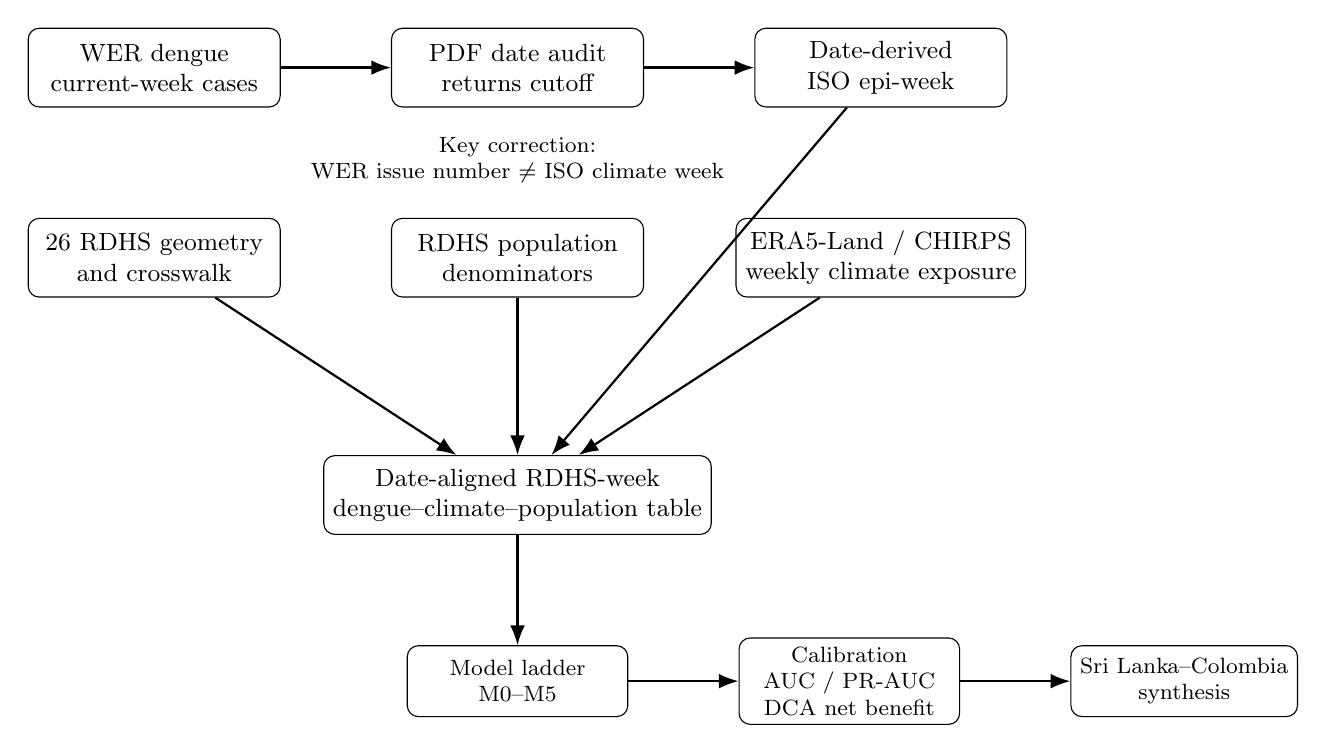
\begin{tikzpicture}[
    node distance=1.4cm and 1.4cm,
    box/.style={
        rectangle,
        rounded corners,
        draw=black,
        align=center,
        minimum width=3.2cm,
        minimum height=1.0cm,
        font=\small
    },
    smallbox/.style={
        rectangle,
        rounded corners,
        draw=black,
        align=center,
        minimum width=2.8cm,
        minimum height=0.9cm,
        font=\footnotesize
    },
    arrow/.style={-{Latex[length=2.5mm]}, thick}
]

\node[box] (wer) {WER dengue\\current-week cases};
\node[box, right=of wer] (date) {PDF date audit\\returns cutoff};
\node[box, right=of date] (iso) {Date-derived\\ISO epi-week};
\node[box, below=of iso] (climate) {ERA5-Land / CHIRPS\\weekly climate exposure};
\node[box, below=of date] (pop) {RDHS population\\denominators};
\node[box, below=of wer] (geom) {26 RDHS geometry\\and crosswalk};

\node[box, below=2.0cm of pop] (linked) {Date-aligned RDHS-week\\dengue--climate--population table};

\node[smallbox, below=of linked] (models) {Model ladder\\M0--M5};
\node[smallbox, right=of models] (eval) {Calibration\\AUC / PR-AUC\\DCA net benefit};
\node[smallbox, right=of eval] (synth) {Sri Lanka--Colombia\\synthesis};

\draw[arrow] (wer) -- (date);
\draw[arrow] (date) -- (iso);
\draw[arrow] (iso) -- (linked);
\draw[arrow] (climate) -- (linked);
\draw[arrow] (pop) -- (linked);
\draw[arrow] (geom) -- (linked);
\draw[arrow] (linked) -- (models);
\draw[arrow] (models) -- (eval);
\draw[arrow] (eval) -- (synth);

\node[align=center, font=\footnotesize, below=0.25cm of date]
(note1) {Key correction:\\WER issue number $\neq$ ISO climate week};

\end{tikzpicture}

\caption{
Study pipeline and WER date-alignment rule. The primary Sri Lanka analysis used a date-derived ISO epidemiological week rather than the stored WER issue number because the issue number was offset from the true surveillance week. This correction prevented climate exposures from being joined to dengue outcomes from the wrong calendar week. The resulting date-aligned RDHS-week table was used for model fitting, calibration assessment, decision-curve analysis, and cross-country interpretation.
}
\label{fig:wer-pipeline}
\end{figure}


\subsection{Primary Sri Lanka model comparison}
\label{subsec:primary-srilanka}

The primary Sri Lanka model ladder compared four models. M0 was a seasonal climatological baseline. M1 was a recent-case autoregressive surveillance baseline using recent dengue incidence and seasonal/RDHS terms. M2 was a climate-only model. M3 was a climate model with seasonality and RDHS fixed effects.

In the held-out 2023--2025 test period, the recent-case surveillance model was the strongest model. M1 had the highest discrimination, lowest Brier score, and highest net benefit at the registered operational reference threshold $p^*=0.30$. Climate-only and climate-plus-seasonality models showed some predictive signal but did not outperform the recent-case surveillance baseline.

\begin{table}[htbp]
\centering
\caption{Primary Sri Lanka test performance, $h=4$, RDHS 75th-percentile alert label.}
\label{tab:srilanka-primary-performance}
\begin{threeparttable}
\small
\begin{tabular}{llrrrrrrrr}
\toprule
Model & Description & AUC & PR-AUC & Brier & CITL & Slope & Mean pred. & Obs. & NB$_{0.30}$ \\
\midrule
M0 & Seasonal climatology & 0.629 & 0.459 & 0.222 & +0.530 & 0.664 & 0.238 & 0.336 & 0.084 \\
M1 & Recent-case surveillance AR & 0.752 & 0.652 & 0.191 & +0.513 & 1.246 & 0.246 & 0.336 & 0.137 \\
M2 & Climate-only & 0.643 & 0.460 & 0.220 & +0.479 & 1.027 & 0.243 & 0.336 & 0.069 \\
M3 & Climate + season + RDHS FE & 0.652 & 0.476 & 0.220 & +0.596 & 0.738 & 0.229 & 0.336 & 0.078 \\
\bottomrule
\end{tabular}
\begin{tablenotes}
\footnotesize
\item Note: CITL denotes calibration-in-the-large. NB$_{0.30}$ denotes net benefit at decision threshold $p^*=0.30$.
\end{tablenotes}
\end{threeparttable}
\end{table}

At the registered threshold $p^*=0.30$, M1 achieved net benefit 0.137, compared with 0.069 for M2 and 0.078 for M3. Thus, the recent-case surveillance model provided substantially higher operational decision value than the climate-only models. Alert-all had lower net benefit than M1 at $p^*=0.30$, and alert-none had net benefit zero.

\subsection{Decision-curve interpretation in the primary Sri Lanka analysis}
\label{subsec:srilanka-dca}

Decision-curve analysis showed that model value was threshold-dependent. At low alert thresholds, alert-all was competitive, as expected when the threshold was much lower than the observed test prevalence. In the mid-to-high threshold region, models provided clearer decision value, and M1 was consistently the strongest model.

\begin{table}[htbp]
\centering
\caption{Sri Lanka net benefit at representative decision thresholds.}
\label{tab:srilanka-net-benefit-thresholds}
\small
\begin{tabular}{rrrrrrr}
\toprule
Threshold $p^*$ & Alert-all & Alert-none & M0 & M1 & M2 & M3 \\
\midrule
0.20 & 0.171 & 0 & 0.161 & 0.185 & 0.164 & 0.147 \\
0.30 & 0.052 & 0 & 0.084 & 0.137 & 0.069 & 0.078 \\
0.34 & -0.005 & 0 & 0.059 & 0.111 & 0.032 & 0.060 \\
0.40 & -0.106 & 0 & 0.025 & 0.083 & 0.012 & 0.039 \\
\bottomrule
\end{tabular}
\end{table}

% =========================================================
% Figure 2
% =========================================================


\begin{figure}[H]
\centering
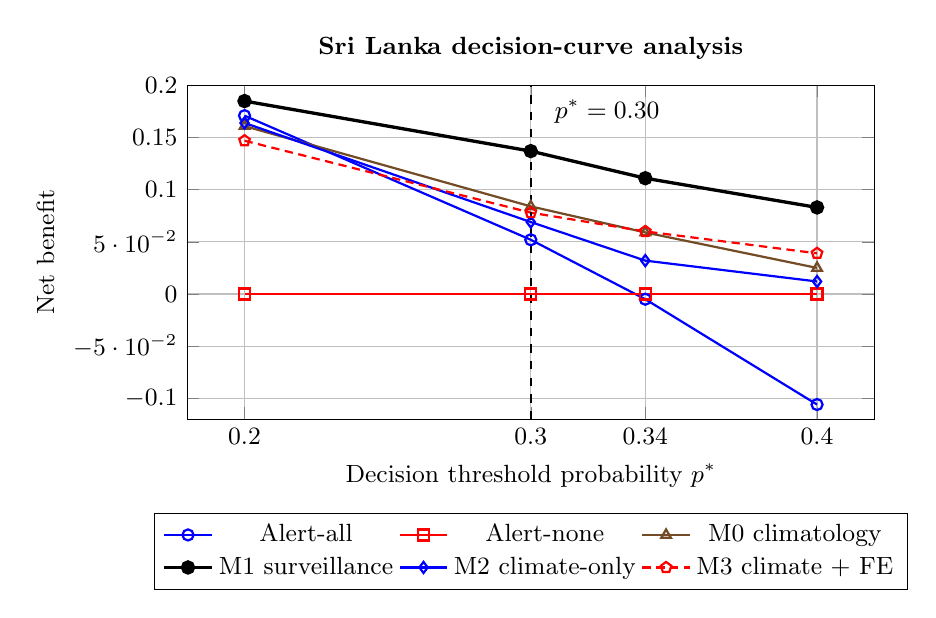
\begin{tikzpicture}
\begin{axis}[
    width=0.85\textwidth,
    height=0.48\textwidth,
    xlabel={Decision threshold probability $p^*$},
    ylabel={Net benefit},
    xmin=0.18, xmax=0.42,
    ymin=-0.12, ymax=0.20,
    xtick={0.20,0.30,0.34,0.40},
    ytick={-0.10,-0.05,0,0.05,0.10,0.15,0.20},
    grid=both,
    legend style={
        at={(0.5,-0.28)},
        anchor=north,
        legend columns=3,
        font=\small
    },
    tick label style={font=\small},
    label style={font=\small},
    title={Sri Lanka decision-curve analysis},
    title style={font=\small\bfseries}
]

% Alert-all
\addplot+[mark=o, thick] coordinates {
    (0.20,0.171)
    (0.30,0.052)
    (0.34,-0.005)
    (0.40,-0.106)
};
\addlegendentry{Alert-all}

% Alert-none
\addplot+[mark=square, thick] coordinates {
    (0.20,0)
    (0.30,0)
    (0.34,0)
    (0.40,0)
};
\addlegendentry{Alert-none}

% M0
\addplot+[mark=triangle, thick] coordinates {
    (0.20,0.161)
    (0.30,0.084)
    (0.34,0.059)
    (0.40,0.025)
};
\addlegendentry{M0 climatology}

% M1
\addplot+[mark=*, very thick] coordinates {
    (0.20,0.185)
    (0.30,0.137)
    (0.34,0.111)
    (0.40,0.083)
};
\addlegendentry{M1 surveillance}

% M2
\addplot+[mark=diamond, thick] coordinates {
    (0.20,0.164)
    (0.30,0.069)
    (0.34,0.032)
    (0.40,0.012)
};
\addlegendentry{M2 climate-only}

% M3
\addplot+[mark=pentagon, thick] coordinates {
    (0.20,0.147)
    (0.30,0.078)
    (0.34,0.060)
    (0.40,0.039)
};
\addlegendentry{M3 climate + FE}

% Vertical line at p*=0.30
\addplot[dashed, thick] coordinates {
    (0.30,-0.12)
    (0.30,0.20)
};

\node[anchor=west, font=\small] at (axis cs:0.305,0.175) {$p^*=0.30$};

\end{axis}
\end{tikzpicture}

\caption{
Sri Lanka decision-curve analysis for the primary $h=4$ RDHS 75th-percentile alert definition. Net benefit is shown at representative threshold probabilities. The recent-case surveillance model (M1) had the highest net benefit across the mid-to-high operational threshold range and at the registered reference threshold $p^*=0.30$. Climate-only models showed some decision value but did not outperform the surveillance baseline.
}
\label{fig:srilanka-dca}
\end{figure}

These results show why the recent-case baseline is essential. Climate-only models may appear to have acceptable discrimination, but when evaluated against the information already available from routine surveillance, their incremental decision value was limited.

The decision-curve results are summarized in Figure~\ref{fig:srilanka-dca}. At the registered reference threshold $p^*=0.30$, the recent-case surveillance model had the highest net benefit among the evaluated models.






\subsection{Calibration drift in the Sri Lanka test period}
\label{subsec:calibration-drift}

All primary models under-predicted risk in the 2023--2025 test period. Calibration-in-the-large was positive for every model: +0.530 for M0, +0.513 for M1, +0.479 for M2, and +0.596 for M3. Mean predicted probabilities were approximately 0.23--0.25, while the observed alert prevalence was 0.336.

This under-prediction is consistent with the training-to-test prevalence shift. The training prevalence was 24.2\%, whereas the test prevalence was 33.6\%. Therefore, the models were trained on a lower-incidence period and evaluated on a higher-incidence period. This finding is important because discrimination alone does not reveal whether predicted probabilities are calibrated well enough for operational alert decisions.

\subsection{Rolling recalibration corrected calibration drift but did not change the main comparison}
\label{subsec:rolling-recalibration}

A time-updated rolling recalibration analysis was conducted to test whether calibration drift could be corrected in an operationally realistic way. The rolling recalibration used only completed prior forecast--outcome pairs available before each prediction week, avoiding leakage from future outcomes.

Rolling 52-week intercept-only recalibration corrected calibration-in-the-large for all four models. M1 CITL improved from +0.513 to +0.020. M0 improved from +0.530 to +0.029, M2 from +0.479 to +0.046, and M3 from +0.596 to +0.087. The 52-week rolling window corrected the base-rate drift better than expanding-window recalibration, which under-corrected because it averaged over earlier lower-incidence years.

\begin{table}[htbp]
\centering
\caption{Calibration-in-the-large before and after time-updated recalibration.}
\label{tab:rolling-recalibration-citl}
\small
\begin{tabular}{lrrrr}
\toprule
Model & Raw CITL & Rolling-52 intercept-only & Rolling-104 intercept-only & Expanding intercept-only \\
\midrule
M0 & +0.530 & +0.029 & +0.137 & +0.338 \\
M1 & +0.513 & +0.020 & +0.111 & +0.325 \\
M2 & +0.479 & +0.046 & +0.155 & +0.314 \\
M3 & +0.596 & +0.087 & +0.204 & +0.394 \\
\bottomrule
\end{tabular}
\end{table}

However, recalibration did not change the model ranking. M1 remained the strongest model under every recalibration method. At $p^*=0.30$, M1 net benefit ranged from 0.124 to 0.142 across recalibration methods, while the climate models remained lower, with maximum climate net benefit approximately 0.085. Thus, calibration drift was operationally correctable, but correcting calibration did not make climate-only models outperform the recent-case surveillance baseline.

% =========================================================
% Figure 3
% =========================================================


\begin{figure}[H]
\centering
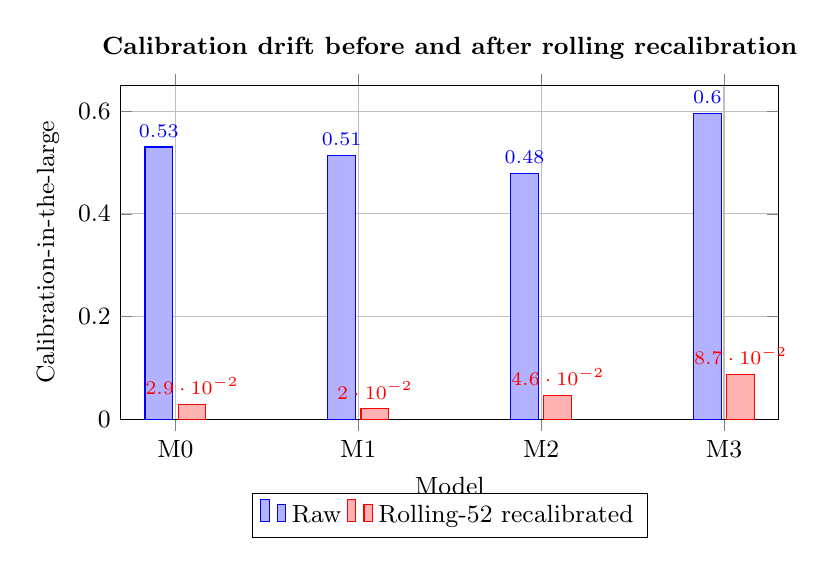
\begin{tikzpicture}
\begin{axis}[
    width=0.82\textwidth,
    height=0.48\textwidth,
    ybar,
    bar width=10pt,
    symbolic x coords={M0,M1,M2,M3},
    xtick=data,
    ymin=0,
    ymax=0.65,
    ylabel={Calibration-in-the-large},
    xlabel={Model},
    legend style={
        at={(0.5,-0.22)},
        anchor=north,
        legend columns=2,
        font=\small
    },
    tick label style={font=\small},
    label style={font=\small},
    title={Calibration drift before and after rolling recalibration},
    title style={font=\small\bfseries},
    grid=both,
    nodes near coords,
    nodes near coords align={vertical},
    every node near coord/.append style={font=\scriptsize}
]

\addplot coordinates {
    (M0,0.530)
    (M1,0.513)
    (M2,0.479)
    (M3,0.596)
};
\addlegendentry{Raw}

\addplot coordinates {
    (M0,0.029)
    (M1,0.020)
    (M2,0.046)
    (M3,0.087)
};
\addlegendentry{Rolling-52 recalibrated}

\end{axis}
\end{tikzpicture}


\caption{
Calibration-in-the-large before and after rolling 52-week intercept-only recalibration
in the Sri Lanka test period. All models showed positive calibration-in-the-large before
recalibration, indicating under-prediction during the higher-incidence 2023--2025 test
period. Rolling recalibration moved calibration-in-the-large close to zero for all models,
showing that temporal base-rate drift was operationally correctable. However, recalibration
did not change the main model comparison: the recent-case surveillance model remained
stronger than the climate-only models on discrimination and decision-curve net benefit.
}

\label{fig:srilanka-calibration}
\end{figure}









\subsection{Sensitivity analyses of linkage, climate lag, and the 2021 anomaly}
\label{subsec:sensitivity-analyses}

Three prespecified sensitivity analyses were conducted for the Sri Lanka $h=4$ / 75th-percentile analysis.

First, the naive v1 literal-week linkage was evaluated. This linkage slightly degraded climate-model performance, as expected under temporal misalignment. M2 AUC decreased to 0.622, compared with 0.643 in the date-aligned v2 analysis. M3 AUC was 0.646 under v1, compared with 0.652 under v2. M1 was essentially unchanged, with AUC 0.753. At $p^*=0.30$, M1 net benefit remained 0.136, whereas M2 and M3 had net benefits of 0.052 and 0.077, respectively.

Second, a climate lag sweep from 0 to 8 weeks showed that climate performance improved modestly when climate variables were lagged by approximately two to four weeks. M2 achieved its best AUC of 0.660 at lag 4 and its best net benefit of 0.088 at lag 2. M3 achieved its best AUC of 0.658 at lag 2 and its best net benefit of 0.088 at lag 4. However, even the best climate lag remained well below M1, which had AUC approximately 0.752 and net benefit 0.137 at $p^*=0.30$.

Third, dropping the late-2021 calendar-anomaly period did not materially change the conclusion. M1 AUC remained 0.753, while M2 and M3 had AUC values of 0.632 and 0.646. M1 also retained the highest net benefit at $p^*=0.30$.

\begin{table}[htbp]
\centering
\caption{Sri Lanka sensitivity summary.}
\label{tab:srilanka-sensitivity-summary}
\small
\begin{tabular}{p{0.23\linewidth}p{0.27\linewidth}p{0.18\linewidth}p{0.18\linewidth}}
\toprule
Sensitivity & Main finding & M1 result & Best climate result \\
\midrule
S1 naive week-number linkage & Climate performance slightly worsened & AUC 0.753; NB$_{0.30}$ 0.136 & M3 AUC 0.646; NB$_{0.30}$ 0.077 \\
S2 climate lag sweep & Climate best at 2--4 week lags & AUC 0.752; NB$_{0.30}$ 0.137 & Best climate AUC 0.660; NB$_{0.30}$ 0.088 \\
S3 drop late-2021 anomaly & Model ordering unchanged & AUC 0.753; NB$_{0.30}$ 0.120 & M3 AUC 0.646; NB$_{0.30}$ 0.066 \\
\bottomrule
\end{tabular}
\end{table}

Together, these sensitivity analyses support the primary conclusion. The result was not an artifact of the linkage rule, contemporaneous climate choice, or the late-2021 calendar anomaly.

\subsection{Canonical R DLNM comparator}
\label{subsec:canonical-dlnm}

To address whether the climate comparator was too simple or depended on a Python approximation, a canonical R \texttt{dlnm} comparator was run using the same primary $h=4$ / 75th-percentile Sri Lanka row set. The canonical R DLNM was statistically indistinguishable from the Python DLNM-style approximation on aggregate metrics. The R-DLNM versus Python-DLNM difference was approximately zero for both AUC and net benefit at $p^*=0.30$, with confidence intervals including zero.

The canonical R DLNM improved over the simple climate logistic models but still did not outperform M1. At $p^*=0.30$, M1 net benefit was 0.1366, compared with 0.1120 for the canonical R DLNM and 0.1112 for the Python-DLNM approximation. The R-DLNM lost to M1 on both discrimination and decision value: $\Delta$AUC was -0.038 with a 95\% confidence interval excluding zero, and $\Delta$NB at $p^*=0.30$ was -0.025 with a 95\% confidence interval excluding zero.

\begin{table}[htbp]
\centering
\caption{Sri Lanka canonical DLNM and hybrid comparison.}
\label{tab:srilanka-dlnm-hybrid}
\small
\begin{tabular}{lrrrr}
\toprule
Model & AUC & NB$_{0.20}$ & NB$_{0.30}$ & NB$_{0.40}$ \\
\midrule
M1 recent-case surveillance & 0.7515 & 0.1849 & 0.1366 & 0.0825 \\
M2 climate-only & 0.6429 & 0.1644 & 0.0687 & 0.0123 \\
M3 climate + season/RDHS & 0.6519 & 0.1469 & 0.0780 & 0.0391 \\
Python DLNM-style climate & 0.7135 & 0.1794 & 0.1112 & 0.0569 \\
Canonical R DLNM climate & 0.7139 & 0.1811 & 0.1120 & 0.0530 \\
M5 hybrid reference & 0.7715 & 0.1944 & 0.1447 & 0.1066 \\
\bottomrule
\end{tabular}
\end{table}

These results show that climate structure does contain predictive information: the canonical R DLNM outperformed the simple climate models. However, the structured climate model still did not provide higher operational value than the recent-case surveillance baseline at the registered threshold.

\subsection{Sri Lanka hybrid model extension}
\label{subsec:srilanka-hybrid}

A hybrid extension tested whether climate could add value when combined with recent surveillance. M4 combined recent-case AR features with a DLNM-style climate cross-basis. M5 added seasonality and RDHS fixed effects.

The hybrid models improved some performance measures relative to M1. M5 had AUC 0.7715, PR-AUC 0.667, Brier score 0.180, and net benefit 0.1447 at $p^*=0.30$, compared with M1 AUC 0.7515, PR-AUC 0.652, Brier score 0.191, and net benefit 0.1366. However, the strict model-winning criterion was not met because the net-benefit improvement over M1 was small and its confidence interval included zero. M5 was therefore interpreted as a near-miss: it improved discrimination and had a higher point estimate for net benefit, but did not provide confirmed operational decision-value gain at the registered threshold.

\begin{table}[htbp]
\centering
\caption{Sri Lanka hybrid model extension.}
\label{tab:srilanka-hybrid}
\small
\begin{tabular}{llrrrrrr}
\toprule
Model & Description & AUC & PR-AUC & Brier & CITL & Slope & NB$_{0.30}$ \\
\midrule
M1 & Recent-case AR baseline & 0.7515 & 0.652 & 0.191 & +0.513 & 1.246 & 0.1366 \\
M4 & AR + DLNM-style climate cross-basis & 0.7643 & 0.641 & 0.187 & +0.449 & 1.225 & 0.1284 \\
M5 & AR + climate + season + RDHS FE & 0.7715 & 0.667 & 0.180 & +0.440 & 1.077 & 0.1447 \\
\bottomrule
\end{tabular}
\end{table}

The Sri Lanka hybrid analysis therefore supports a cautious interpretation. Climate information may add some signal when combined with recent surveillance, but the registered operational evidence did not confirm a robust model-winning climate advantage.

\subsection{Label and horizon robustness in Sri Lanka}
\label{subsec:srilanka-label-horizon}

The Sri Lanka analysis was further evaluated across label thresholds and forecast horizons. Ten cells were considered: 75th- and 90th-percentile alert definitions crossed with horizons $h=1,2,4,8,$ and 12 weeks. Stop rules passed in all cells, and the 90th-percentile label was not sparse, with approximately 399--426 test events.

M1 net benefit at $p^*=0.30$ was highest in all 10 label-horizon cells. At the 75th-percentile label, M1 AUC declined as the forecast horizon increased: 0.843 at $h=1$, 0.810 at $h=2$, 0.751 at $h=4$, 0.679 at $h=8$, and 0.646 at $h=12$. Climate models were flatter across horizons and became competitive on discrimination at longer leads. For example, climate models exceeded M1 AUC in selected long-horizon cells, including 75th-percentile $h=12$ and 90th-percentile $h=8$ or $h=12$. However, these discrimination crossovers did not overturn the registered net-benefit result at $p^*=0.30$.

This distinction is central to the paper. Climate may become more competitive on AUC at longer horizons, but operational decision value at the registered threshold remained strongest for the recent-case surveillance model in the Sri Lanka analysis.
The horizon and alert-label robustness results are summarized in Figure~\ref{fig:srilanka-horizon-robustness}.
Although M1 discrimination declined with longer forecast horizons, M1 retained the highest net benefit at $p^*=0.30$ across all tested label-horizon combinations.



% =========================================================
% Figure 4
% =========================================================
\begin{figure}[!htbp]
\centering

% ---------------- Panel A ----------------
\begin{subfigure}[t]{0.48\textwidth}
\centering
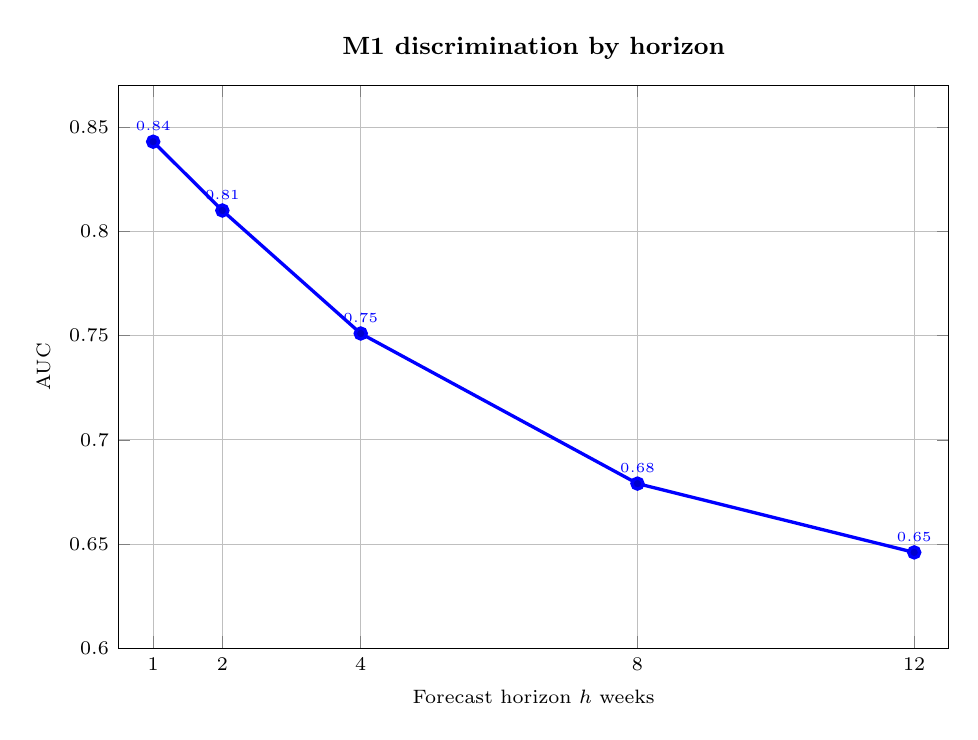
\begin{tikzpicture}
\begin{axis}[
    width=\linewidth,
    height=0.72\linewidth,
    xlabel={Forecast horizon $h$ weeks},
    ylabel={AUC},
    xmin=0.5, xmax=12.5,
    ymin=0.60, ymax=0.87,
    xtick={1,2,4,8,12},
    ytick={0.60,0.65,0.70,0.75,0.80,0.85},
    grid=both,
    tick label style={font=\scriptsize},
    label style={font=\scriptsize},
    title={M1 discrimination by horizon},
    title style={font=\small\bfseries},
    nodes near coords,
    every node near coord/.append style={font=\tiny},
]
\addplot+[mark=*, very thick] coordinates {
    (1,0.843)
    (2,0.810)
    (4,0.751)
    (8,0.679)
    (12,0.646)
};
\end{axis}
\end{tikzpicture}
\caption{AUC of the recent-case surveillance model.}
\label{fig:horizon-auc}
\end{subfigure}
\hfill
% ---------------- Panel B ----------------
\begin{subfigure}[t]{0.48\textwidth}
\centering
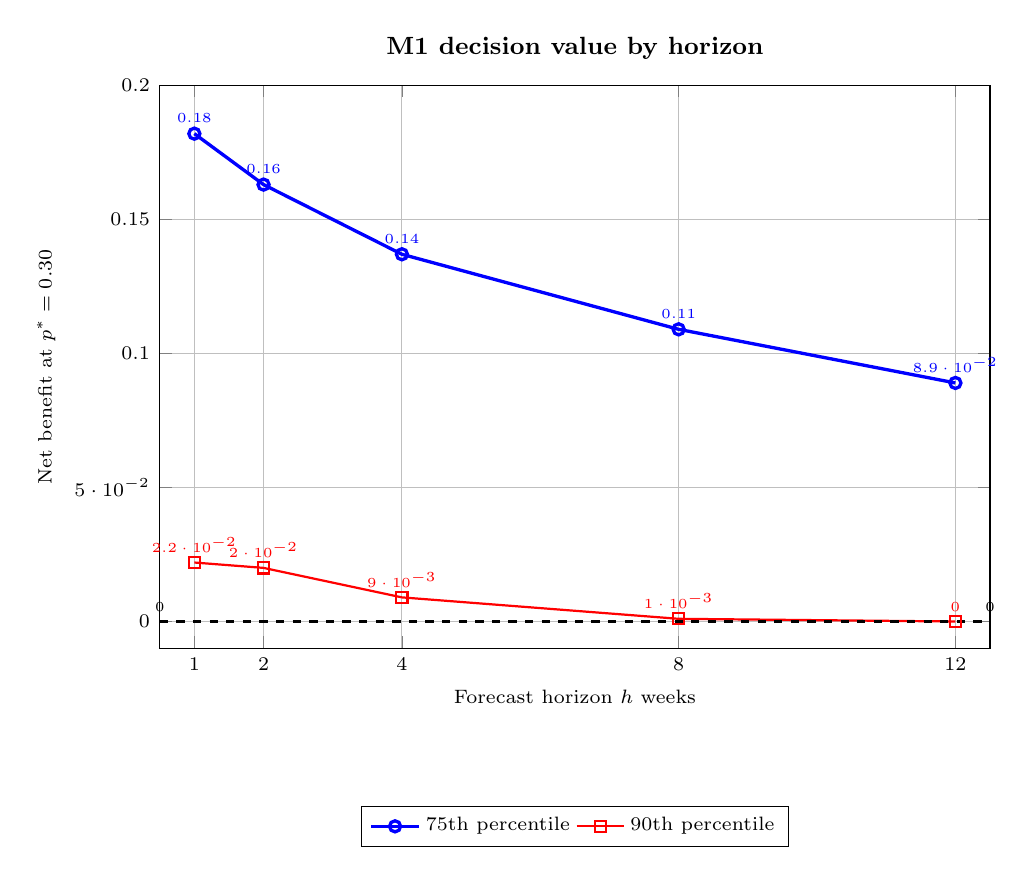
\begin{tikzpicture}
\begin{axis}[
    width=\linewidth,
    height=0.72\linewidth,
    xlabel={Forecast horizon $h$ weeks},
    ylabel={Net benefit at $p^*=0.30$},
    xmin=0.5, xmax=12.5,
    ymin=-0.01, ymax=0.20,
    xtick={1,2,4,8,12},
    ytick={0,0.05,0.10,0.15,0.20},
    grid=both,
    tick label style={font=\scriptsize},
    label style={font=\scriptsize},
    title={M1 decision value by horizon},
    title style={font=\small\bfseries},
    legend style={
        at={(0.5,-0.28)},
        anchor=north,
        legend columns=2,
        font=\scriptsize
    },
    nodes near coords,
    every node near coord/.append style={font=\tiny},
]
\addplot+[mark=o, very thick] coordinates {
    (1,0.182)
    (2,0.163)
    (4,0.137)
    (8,0.109)
    (12,0.089)
};
\addlegendentry{75th percentile}

\addplot+[mark=square, thick] coordinates {
    (1,0.022)
    (2,0.020)
    (4,0.009)
    (8,0.001)
    (12,0.000)
};
\addlegendentry{90th percentile}

\addplot[dashed, thick] coordinates {
    (0.5,0)
    (12.5,0)
};

\end{axis}
\end{tikzpicture}
\caption{Net benefit of the recent-case surveillance model.}
\label{fig:horizon-nb}
\end{subfigure}

\caption{
Sri Lanka robustness of the recent-case surveillance benchmark across forecast horizons and alert-label definitions.
Panel A shows that discrimination for the M1 recent-case surveillance model declined as the forecast horizon increased under the 75th-percentile alert definition.
Panel B shows net benefit at the registered decision threshold $p^*=0.30$ for the 75th- and 90th-percentile alert definitions.
M1 had the highest net benefit at $p^*=0.30$ in all 10 label-horizon cells, supporting the conclusion that recent surveillance remained a hard-to-beat operational benchmark even when discrimination became less favorable at longer horizons.
}
\label{fig:srilanka-horizon-robustness}
\end{figure}
\FloatBarrier

\subsection{Targeted value of climate information in Sri Lanka}
\label{subsec:targeted-value}

A targeted value analysis examined whether the hybrid climate-surveillance model M5 added net benefit over M1 in train-defined regimes. Regimes were defined using training-period incidence and lag-1 autocorrelation. The primary estimand was $\Delta$NB(M5$-$M1) at $p^*=0.30$.

In the all-test reference set, $\Delta$NB(M5$-$M1) was +0.0081, with a 95\% confidence interval from -0.0012 to 0.0181. Thus, the overall Sri Lanka hybrid advantage at $p^*=0.30$ did not exclude zero. In the adequately powered single-axis regimes, no confidence interval excluded zero. The high-incidence regime had $\Delta$NB +0.0128, but the interval crossed zero. The weak-AR and strong-AR regimes also had positive point estimates, but their intervals crossed zero.

One combined regime, high-incidence plus strong-autocorrelation, showed a positive $\Delta$NB of +0.0202 with a 95\% confidence interval from 0.0038 to 0.0370. However, this cell included only eight RDHS clusters and was flagged as underpowered. Therefore, this result was treated as hypothesis-generating rather than confirmatory.

\begin{table}[htbp]
\centering
\caption{Sri Lanka targeted value of climate, $\Delta$NB(M5$-$M1) at $p^*=0.30$.}
\label{tab:srilanka-targeted-value}
\small
\begin{tabular}{lrrrrll}
\toprule
Regime & Test $n$ & Events & RDHS & $\Delta$NB & 95\% CI & Interpretation \\
\midrule
All & 3926 & 1321 & 26 & +0.0081 & [-0.0012, 0.0181] & Positive point estimate, not confirmed \\
Low incidence & 1963 & 715 & 13 & +0.0034 & [-0.0100, 0.0181] & Not confirmed \\
High incidence & 1963 & 606 & 13 & +0.0128 & [-0.0009, 0.0264] & Near-miss, not confirmed \\
Weak AR & 1963 & 629 & 13 & +0.0079 & [-0.0039, 0.0213] & Not confirmed \\
Strong AR & 1963 & 692 & 13 & +0.0083 & [-0.0071, 0.0234] & Not confirmed \\
Low + weak AR & 1208 & 477 & 8 & +0.0122 & [-0.0032, 0.0295] & Underpowered \\
Low + strong AR & 755 & 238 & 5 & -0.0108 & [-0.0301, 0.0098] & Underpowered \\
High + weak AR & 755 & 152 & 5 & +0.0010 & [-0.0142, 0.0170] & Underpowered \\
High + strong AR & 1208 & 454 & 8 & +0.0202 & [0.0038, 0.0370] & Positive but underpowered \\
\bottomrule
\end{tabular}
\end{table}

At other thresholds, the hybrid advantage was stronger. At $p^*=0.40$, the overall $\Delta$NB was +0.0241 with a confidence interval excluding zero, and several powered regimes also excluded zero. However, because $p^*=0.30$ was the registered primary threshold, the $p^*=0.40$ finding was interpreted as threshold-dependent supportive evidence rather than the primary conclusion.

\subsection{Colombia external framework replication}
\label{subsec:colombia-replication}

The Colombia analysis replicated the decision-evaluation framework using a local refit rather than transferring Sri Lanka coefficients. The primary Colombia $h=4$ analysis used a common-complete M1--M5 row set with 13,361 test observations and test prevalence 0.375. The model ladder included recent-case surveillance, climate-only models, and hybrid climate-surveillance models.

The Colombia result partly replicated and partly extended the Sri Lanka pattern. As in Sri Lanka, climate-only models were weak relative to recent surveillance. M2 had AUC 0.556 and M3 had AUC 0.564, compared with M1 AUC 0.685. Climate-only models were also operationally weak at $p^*=0.30$.

Unlike Sri Lanka, however, the hybrid models showed confirmed incremental value over recent surveillance. M5 had AUC 0.726 and net benefit 0.136 at $p^*=0.30$, compared with M1 AUC 0.685 and net benefit 0.117. The M5 versus M1 difference was confirmed by municipality-cluster bootstrap: $\Delta$AUC was +0.040 with 95\% CI [0.024, 0.058], and $\Delta$NB at $p^*=0.30$ was +0.018 with 95\% CI [0.012, 0.026].

\begin{table}[htbp]
\centering
\caption{Colombia $h=4$ primary test performance.}
\label{tab:colombia-primary-performance}
\small
\begin{tabular}{llrrr}
\toprule
Model & Description & AUC & NB$_{0.30}$ & Interpretation \\
\midrule
M1 & Recent-case surveillance & 0.685 & 0.117 & Strong surveillance benchmark \\
M2 & Climate-only & 0.556 & Not competitive & Weak standalone climate signal \\
M3 & Climate + seasonality & 0.564 & Not competitive & Weak standalone climate signal \\
M4 & Hybrid without full fixed effects & 0.699 & 0.129 & Modest hybrid improvement \\
M5 & Hybrid climate + surveillance & 0.726 & 0.136 & Confirmed modest improvement over M1 \\
\bottomrule
\end{tabular}
\end{table}
%------------------------------------------------------------------------
% figure 5
%------------------------------------------------------------------
\begin{figure}[!htbp]
\centering

% ---------------- Panel A: AUC ----------------
\begin{subfigure}[t]{0.48\textwidth}
\centering
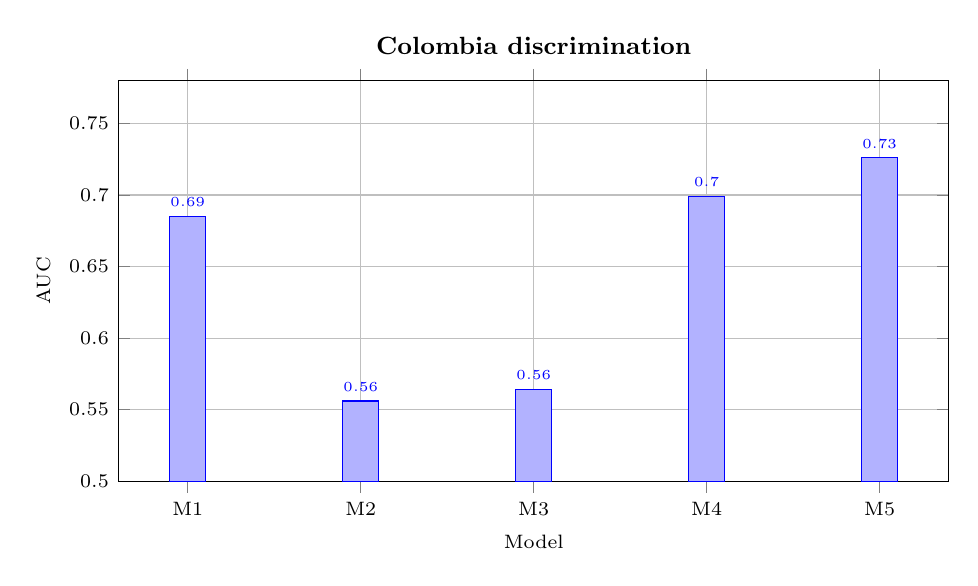
\begin{tikzpicture}
\begin{axis}[
    width=\linewidth,
    height=0.55\linewidth,
    ybar,
    bar width=13pt,
    symbolic x coords={M1,M2,M3,M4,M5},
    xtick=data,
    ymin=0.50,
    ymax=0.78,
    ylabel={AUC},
    xlabel={Model},
    grid=both,
    tick label style={font=\scriptsize},
    label style={font=\scriptsize},
    title={Colombia discrimination},
    title style={font=\small\bfseries},
    nodes near coords,
    nodes near coords align={vertical},
    every node near coord/.append style={font=\tiny}
]
\addplot coordinates {
    (M1,0.685)
    (M2,0.556)
    (M3,0.564)
    (M4,0.699)
    (M5,0.726)
};
\end{axis}
\end{tikzpicture}
\caption{AUC by model.}
\label{fig:colombia-auc}
\end{subfigure}
\hfill
% ---------------- Panel B: Net benefit ----------------
\begin{subfigure}[t]{0.48\textwidth}
\centering
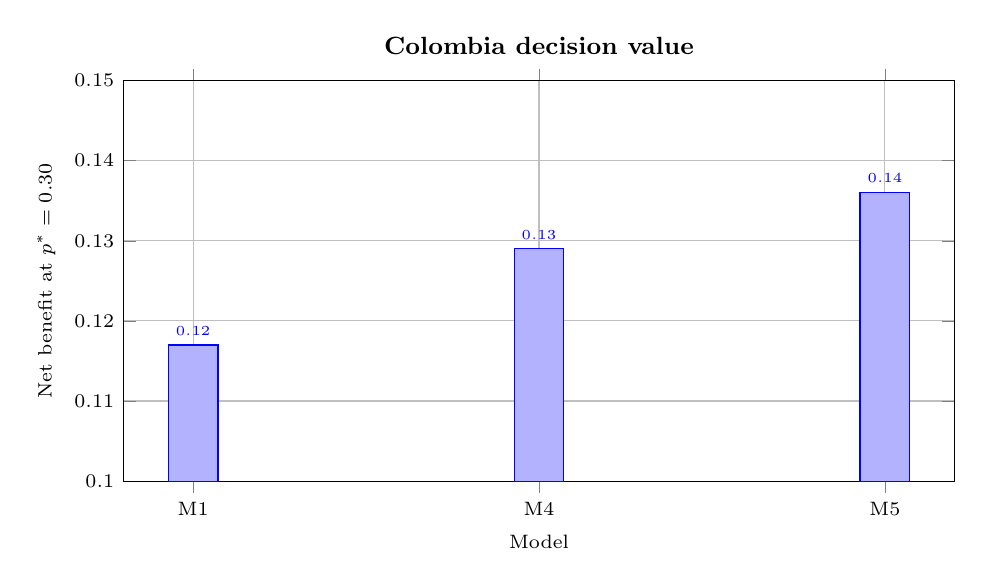
\begin{tikzpicture}
\begin{axis}[
    width=\linewidth,
    height=0.55\linewidth,
    ybar,
    bar width=18pt,
    symbolic x coords={M1,M4,M5},
    xtick=data,
    ymin=0.10,
    ymax=0.15,
    ylabel={Net benefit at $p^*=0.30$},
    xlabel={Model},
    grid=both,
    tick label style={font=\scriptsize},
    label style={font=\scriptsize},
    title={Colombia decision value},
    title style={font=\small\bfseries},
    nodes near coords,
    nodes near coords align={vertical},
    every node near coord/.append style={font=\tiny}
]
\addplot coordinates {
    (M1,0.117)
    (M4,0.129)
    (M5,0.136)
};
\end{axis}
\end{tikzpicture}
\caption{Net benefit at $p^*=0.30$.}
\label{fig:colombia-nb}
\end{subfigure}

\caption{
Colombia external framework replication.
Panel A shows discrimination across the model ladder. Climate-only models M2 and M3 had weak discrimination relative to the recent-case surveillance baseline M1, whereas the hybrid model M5 had the highest AUC.
Panel B shows net benefit at the operational reference threshold $p^*=0.30$ for the surveillance and hybrid models. M5 improved over M1 by $\Delta$NB = +0.018, with a municipality-cluster bootstrap 95\% confidence interval excluding zero.
This supports the interpretation that climate information was most useful as a modest hybrid increment rather than as a standalone replacement for recent surveillance.
}
\label{fig:colombia-hybrid}
\end{figure}





In the secondary full climate-only row set, M2 and M3 remained weak, with AUC values around 0.532 and 0.546 and net benefit near zero at $p^*=0.30$. This supports the conclusion that climate-only weakness was not simply an artifact of the common-complete head-to-head row set.

The Colombia result should not be interpreted as global validation or deployment readiness. The test period included COVID-era years and showed over-prediction in calibration. Nevertheless, the within-test comparison between M5 and M1 supports the conclusion that climate can add modest operational value when integrated with recent surveillance.


\subsection{Colombia horizon sensitivity}
\label{subsec:colombia-horizon}

The Colombia horizon sensitivity analysis tested whether the hybrid climate-surveillance increment increased at longer lead times. It did not. The M5 versus M1 net-benefit advantage was approximately flat across $h=1$ to $h=8$ and slightly lower at $h=12$. $\Delta$NB(M5$-$M1) was approximately +0.015 to +0.019 across $h=1$--8 and approximately +0.014 at $h=12$. The $\Delta$AUC advantage also decreased at longer horizons, from approximately +0.040 at $h \leq 4$ to approximately +0.024 at $h=12$.

However, the hybrid advantage was consistent: M5 $\Delta$NB confidence intervals excluded zero at every tested horizon. Thus, the Colombia $h=4$ hybrid finding was not a single-horizon artifact. Climate-only models remained weak across horizons, and absolute predictability declined by $h=12$, where both M1 and M5 approached low net benefit.

The horizon sensitivity therefore supports a cautious conclusion. Hybrid climate-surveillance models can add a modest, consistent increment, but the evidence does not support the stronger claim that climate value increases across the 1--12 week horizon range.


\subsection{Cross-country synthesis}
The cross-country interpretation is summarized in Figure~\ref{fig:cross-country-synthesis}.
\begin{figure}[!htbp]
\centering
\scriptsize
\renewcommand{\arraystretch}{1.08}
\begin{tabular}{p{0.44\textwidth}p{0.44\textwidth}}
\toprule
\textbf{Sri Lanka} & \textbf{Colombia} \\
\midrule

\textbf{Primary setting:} RDHS-week evaluation, 2018--2025.
&
\textbf{Replication setting:} external framework replication using local refitting.
\\[0.08cm]

\textbf{Surveillance benchmark:} recent-case surveillance was difficult to beat.
&
\textbf{Surveillance benchmark:} recent-case surveillance was also a strong comparator.
\\[0.08cm]

\textbf{Climate-only models:} limited standalone operational value.
&
\textbf{Climate-only models:} weak relative to recent surveillance.
\\[0.08cm]

\textbf{Hybrid result:} M5 showed a positive point estimate but was not confirmed at the registered threshold $p^*=0.30$.
&
\textbf{Hybrid result:} M5 showed a modest but confirmed improvement over M1.
\\[0.08cm]

\textbf{Calibration:} temporal calibration drift was present but correctable by rolling recalibration.
&
\textbf{Horizon pattern:} hybrid gain was stable but did not increase across $h=1$--12 weeks.
\\

\bottomrule
\end{tabular}

\vspace{0.25cm}

\fbox{
\begin{minipage}{0.86\textwidth}
\centering
\footnotesize
\textbf{Cross-country interpretation:}
Climate information was not a standalone replacement for routine dengue surveillance.
Its operational value was most defensible as a modest, hybrid-specific, and setting-dependent increment.
Calibration and decision-curve net benefit should be reported before claims of climate-EWS value are made.
\end{minipage}
}

\caption{
Cross-country synthesis of the decision-evaluation results. Sri Lanka showed that climate value was not guaranteed at the registered threshold, whereas Colombia showed that climate could add modest but statistically supported value when integrated with recent surveillance.
}
\label{fig:cross-country-synthesis}
\end{figure}

Across Sri Lanka and Colombia, recent dengue surveillance was a strong benchmark. Climate-only models did not outperform recent surveillance in either setting. In Sri Lanka, even canonical DLNM climate structure did not beat recent surveillance, and the hybrid model showed only a near-miss at the registered threshold. In Colombia, the hybrid model produced a confirmed but modest net-benefit improvement over recent surveillance.

These findings are complementary rather than contradictory. Sri Lanka shows that climate value is not guaranteed and may be threshold-, regime-, and setting-dependent. Colombia shows that climate can add operational value when used as an incremental signal within a hybrid model. Together, the results support evaluating climate information as an add-on to surveillance rather than as a standalone replacement.



\subsection{Main results summary}
\label{subsec:main-results-summary}

The overall result is not that climate-only dengue early-warning models outperform surveillance. Instead, the analysis shows four main findings.

First, recent dengue surveillance is a hard-to-beat operational benchmark, especially at short-to-medium forecast horizons. Second, climate-only models have limited standalone operational value when compared against recent surveillance. Third, calibration drift can be substantial under temporal base-rate shifts, but simple rolling recalibration can correct calibration-in-the-large. Fourth, climate information may add modest value when integrated with recent surveillance, but this value is setting-dependent and should be demonstrated using decision-curve net benefit, not AUC alone.

Therefore, climate-informed dengue early-warning systems should be benchmarked against recent surveillance and evaluated with calibration, recalibration, and decision-curve net benefit before claims of operational value are made.


\section{Discussion}
\label{sec:discussion}

\subsection{Principal findings}
\label{subsec:principal-findings}

This study evaluated climate-informed dengue early-warning models using a surveillance-benchmarked, calibration-aware, decision-analytic framework. The main finding is that recent dengue surveillance is a hard-to-beat operational benchmark. In Sri Lanka, climate-only models did not outperform the recent-case surveillance baseline at the primary four-week horizon or at the registered decision threshold. Structured climate models captured additional climate signal, and hybrid models improved some discrimination and point estimates of net benefit, but the Sri Lanka hybrid improvement was not confirmed at the registered threshold. In Colombia, climate-only models were also weak relative to surveillance, but the hybrid climate--surveillance model produced a modest and statistically supported improvement over surveillance alone.

These findings support a cautious interpretation of climate-informed dengue early warning. Climate information should not be treated as a standalone replacement for routine surveillance. Its operational value is more defensible as an incremental signal within hybrid models that also include recent dengue incidence. Even then, the magnitude of improvement was modest and setting-dependent.

\subsection{Recent surveillance is a strong operational benchmark}
\label{subsec:surveillance-benchmark-discussion}

A central implication of this study is that climate-informed early-warning systems should be benchmarked against recent surveillance, not only against climatology, alert-all, alert-none, or weak null models. Dengue incidence is temporally autocorrelated, so recent case counts contain strong short-term information about near-future risk. In the Sri Lanka analysis, the recent-case surveillance model outperformed climate-only models on discrimination and decision-curve net benefit at the primary operational horizon. This result persisted across linkage, lag, anomaly, label, horizon, and recalibration analyses.

This does not mean climate is irrelevant to dengue transmission. Climate affects mosquito and virus dynamics, and climate models can capture meaningful environmental risk. Rather, the operational question is whether climate improves decisions beyond information already available from recent case surveillance. In short-to-medium operational horizons, recent surveillance can already summarize many upstream processes, including climate effects, human behavior, immunity, reporting, and local transmission dynamics. Therefore, climate-only models face a demanding but appropriate benchmark.

\subsection{Climate-only models had limited standalone decision value}
\label{subsec:climate-only-discussion}

Climate-only models showed some signal but limited standalone operational value. In Sri Lanka, simple climate models were weaker than the recent-case baseline, and a canonical distributed-lag nonlinear climate comparator improved over simple climate models but still did not outperform recent surveillance at the registered decision threshold. In Colombia, climate-only models were also weak relative to recent surveillance. This cross-setting pattern suggests that climate-only dengue early-warning models may be insufficient for operational deployment when recent case surveillance is available.

This finding should not be interpreted as evidence that climate has no role in dengue early warning. Instead, it shows that climate-only models can be operationally weak when evaluated against a strong surveillance comparator. Climate may be more useful at longer horizons, in areas with weaker surveillance, during unusual climatic conditions, or as part of a hybrid model. The present results therefore argue against climate-only superiority, not against climate-informed early warning in general.

\subsection{Hybrid climate--surveillance models can add modest, setting-dependent value}
\label{subsec:hybrid-discussion}

The hybrid results are the most important nuance of the study. In Sri Lanka, the hybrid model improved discrimination and had a higher point estimate of net benefit than the surveillance-only model, but the net-benefit confidence interval at the registered threshold did not exclude zero. Targeted-value analysis suggested possible benefit in some regimes and at higher decision thresholds, but these signals were not confirmed in adequately powered primary comparisons.

In Colombia, the hybrid climate--surveillance model produced a confirmed improvement over recent surveillance. The improvement was statistically supported but modest in magnitude. Horizon sensitivity showed that the hybrid gain was stable across tested horizons but did not increase strongly with lead time. Therefore, the Colombia result supports climate as a complementary signal, but not as evidence of a large or universal climate advantage.

Together, the two settings suggest that climate value is conditional. It depends on geography, surveillance dynamics, incidence regime, decision threshold, model specification, and alert definition. The most defensible claim is therefore not that climate-informed models outperform surveillance, but that climate may add modest operational value when integrated with recent surveillance and evaluated in the appropriate setting.

\subsection{Calibration drift is operationally important}
\label{subsec:calibration-discussion}

A second major finding is that calibration drift can materially affect dengue early-warning interpretation. In the Sri Lanka test period, all models under-predicted alert risk because the held-out period had higher alert prevalence than the training period. This is a realistic deployment problem: dengue incidence can shift between training and deployment periods because of changing immunity, serotype dynamics, reporting patterns, vector control, climate anomalies, or broader social conditions.

Rolling 52-week recalibration corrected calibration-in-the-large for all models, showing that temporal base-rate drift was operationally correctable. However, recalibration did not change the main model comparison: recent surveillance remained stronger than climate-only models. This distinction matters. The climate-only models did not lose simply because of poor calibration; even after correcting calibration drift, they did not provide higher operational decision value than recent surveillance.

The practical implication is that dengue early-warning systems should include ongoing calibration monitoring. Static model evaluation is not enough. A model that was calibrated during development can become miscalibrated during deployment. Simple time-updated recalibration may be an effective operational safeguard, but it should be evaluated explicitly rather than assumed.

\subsection{Why decision-curve analysis changes the evaluation}
\label{subsec:dca-discussion}

Discrimination metrics alone were insufficient to summarize operational value. AUC measures ranking, not whether predicted probabilities support better public-health decisions at a given threshold. A model can have acceptable AUC but still be poorly calibrated or produce lower net benefit than a simpler comparator.

Decision-curve analysis directly evaluates whether a model improves threshold-based alert decisions after accounting for false-positive alert cost. This is especially important for dengue early warning because alert decisions have practical consequences: vector-control mobilization, staff time, public communication, and potential response fatigue. A model should therefore be evaluated by whether it improves alert decisions compared with realistic alternatives, including recent surveillance.

In this study, DCA clarified the main operational pattern. Climate-only models showed some discrimination but limited decision value against surveillance. Hybrid models could add value, but the gain was modest and setting-dependent. This interpretation would be less clear from AUC alone.

\subsection{Data-linkage and geospatial contributions}
\label{subsec:data-linkage-discussion}

The study also highlights the importance of careful data alignment. In Sri Lanka, the WER issue number did not always correspond to the true ISO climate week. A naive week-number join would have misaligned dengue outcomes and climate exposures by one to two weeks. Because climate-lag relationships are sensitive to timing, this kind of linkage error can bias conclusions about climate signal.

The RDHS spatial backbone, Ampara--Kalmunai split, population denominators, and adjacency graph provided a defensible spatial structure for the analysis. These steps are not merely administrative. Incidence calculations, climate aggregation, spatial comparisons, and calibration assessment all depend on the spatial and temporal units being correctly defined. A major methodological lesson is that climate-informed early-warning evaluations should treat data alignment and spatial support as core parts of the analysis rather than as preprocessing details.

\subsection{Public-health implications}
\label{subsec:public-health-implications}

For public-health agencies, the results suggest a practical evaluation hierarchy. First, any climate-informed dengue early-warning system should be compared with recent surveillance. Second, predicted probabilities should be evaluated for calibration, not only discrimination. Third, decision-curve net benefit should be reported across plausible operational thresholds. Fourth, recalibration should be considered as part of deployment monitoring.

The findings also suggest that climate should be positioned realistically. Climate-only models may be attractive because they appear to offer earlier warning, but their standalone operational value may be limited when surveillance data are available. Hybrid systems are more plausible: recent cases capture current transmission momentum, while climate may add information about environmental suitability or future amplification. The value of such hybrid systems should be quantified rather than assumed.

\subsection{Strengths}
\label{subsec:strengths}

This study has several strengths. First, it used a recent-surveillance baseline as the main comparator, making the evaluation operationally realistic. Second, it combined discrimination, calibration, recalibration, and decision-curve net benefit rather than relying on AUC alone. Third, the Sri Lanka analysis used a carefully audited temporal linkage between dengue reports and climate weeks. Fourth, the spatial backbone and population denominators were constructed with explicit quality control. Fifth, the analysis included robustness checks for linkage, climate lag, calendar anomaly handling, label threshold, forecast horizon, structured climate modeling, hybrid modeling, recalibration, and targeted value. Sixth, the Colombia replication tested whether the framework produced similar qualitative conclusions in a second setting using local refitting.

\subsection{Limitations}
\label{subsec:limitations}

The study also has important limitations. First, it was retrospective. The models were evaluated on held-out historical data, not in prospective real-time deployment. Therefore, the results should not be interpreted as deployment-ready performance.

Second, the alert labels were based on percentile thresholds rather than official operational outbreak declarations. Percentile-based labels are useful for consistent evaluation across spatial units, but they may not fully match public-health decision rules. Results may differ under alternative outbreak definitions.

Third, the primary Sri Lanka validation used a temporal holdout rather than a full prospective rolling-origin and spatial-block validation design. Although the temporal holdout was out-of-sample, a future confirmatory study should evaluate performance under rolling-origin deployment conditions and account more fully for spatial dependence.

Fourth, the analysis did not include serotype, immunity, entomological surveillance, mobility, vector-control activities, socioeconomic covariates, or reporting-delay adjustments. These omitted factors may explain variation in dengue risk and may affect the apparent incremental value of climate.

Fifth, climate exposure was aggregated to administrative spatial units. RDHS- or municipality-level aggregation may mask within-unit heterogeneity in urbanization, elevation, land cover, and microclimate. Although the geospatial backbone was carefully constructed, change-of-support and modifiable-areal-unit issues remain relevant.

Sixth, the Colombia analysis was an external framework replication, not global validation. The models were refit locally, and the findings should not be interpreted as evidence that the same coefficients or thresholds would transport to other countries. Additional settings are needed before making broader claims.

Seventh, the hybrid gains were modest. Even when statistically supported, modest net-benefit improvements may or may not be sufficient to change practice depending on local response costs, available resources, and tolerance for false alerts. This study did not conduct a full cost-effectiveness analysis.

\subsection{Future work}
\label{subsec:future-work}

Future work should evaluate the framework prospectively under real-time reporting conditions. This would require accounting for reporting delays, data revisions, and the operational timing of vector-control response. Future studies should also test whether hybrid climate--surveillance value is larger in settings with weaker surveillance, stronger climate seasonality, longer reporting delays, or different dengue transmission regimes.

Further work should incorporate additional covariates such as serotype circulation, immunity proxies, human mobility, vector indices, land cover, and intervention history. Spatially explicit evaluation could also identify where climate information is most useful and whether targeted hybrid models improve local decisions.

Finally, future research should connect decision-curve thresholds to explicit public-health costs and losses. This would allow net-benefit results to be interpreted more directly in terms of intervention cost, missed-outbreak loss, and health-system capacity.

\subsection{Conclusion}
\label{subsec:discussion-conclusion}

This study does not show that climate-only dengue early-warning models outperform recent surveillance. Instead, it shows that recent dengue surveillance is a strong operational benchmark, climate-only models have limited standalone decision value, and climate information may add modest, setting-dependent value when integrated with recent surveillance. Calibration drift was substantial but correctable by time-updated recalibration. Operational evaluation of dengue early-warning systems should therefore report calibration and decision-curve net benefit against recent-surveillance baselines before claims of climate-informed value are made.














\bibliographystyle{apalike}
\bibliography{references}





\end{document}
